\documentclass{article} 
\usepackage{CJK}
\usepackage{561project,times}
\usepackage{hyperref}
\usepackage{url}
\usepackage{graphicx}
\usepackage{caption}
\usepackage{subfig}
\usepackage{bm}
\usepackage{float}
\usepackage{mathrsfs}
\usepackage{bbm}
\usepackage{amsmath,amsthm,amsfonts,amssymb,amscd}
\usepackage{booktabs}
\newcommand{\beq}{\vspace{0mm}\begin{equation}}
\newcommand{\eeq}{\vspace{0mm}\end{equation}}
\newcommand{\beqs}{\vspace{0mm}\begin{eqnarray}}
\newcommand{\eeqs}{\vspace{0mm}\end{eqnarray}}
\newcommand{\barr}{\begin{array}}
\newcommand{\earr}{\end{array}}
\newcommand{\Amat}[0]{{{\bf A}}}
\newcommand{\Bmat}{{\bf B}}
\newcommand{\Cmat}{{\bf C}}
\newcommand{\Dmat}{{\bf D}}
\newcommand{\Emat}[0]{{{\bf E}}}
\newcommand{\Fmat}[0]{{{\bf F}}\xspace}
\newcommand{\Gmat}{{\bf G}}
\newcommand{\Hmat}{{\bf H}}
\newcommand{\Imat}{{\bf I}}
\newcommand{\Jmat}[0]{{{\bf J}}\xspace}
\newcommand{\Kmat}[0]{{{\bf K}}\xspace}
\newcommand{\Lmat}[0]{{{\bf L}}}
\newcommand{\Mmat}{{\bf M}}
\newcommand{\Nmat}[0]{{{\bf N}}\xspace}
\newcommand{\Omat}[0]{{{\bf O}}}
\newcommand{\Pmat}{{\bf P}}
\newcommand{\Qmat}[0]{{{\bf Q}}\xspace}
\newcommand{\Rmat}[0]{{{\bf R}}}
\newcommand{\Smat}[0]{{{\bf S}}}
\newcommand{\Tmat}[0]{{{\bf T}}}
\newcommand{\Umat}[0]{{{\bf U}}}
\newcommand{\Vmat}[0]{{{\bf V}}}
\newcommand{\Wmat}[0]{{{\bf W}}}
\newcommand{\Xmat}[0]{{{\bf X}}}
\newcommand{\Ymat}{{\bf Y}}
\newcommand{\Zmat}{{\bf Z}}
\newcommand{\av}[0]{{\boldsymbol{a}}}
\newcommand{\bv}[0]{{\boldsymbol{b}}}
\newcommand{\cv}[0]{{\boldsymbol{c}}}
\newcommand{\dv}{\boldsymbol{d}}
\newcommand{\ev}[0]{{\boldsymbol{e}}\xspace}
\newcommand{\fv}[0]{{\boldsymbol{f}}\xspace}
\newcommand{\gv}[0]{{\boldsymbol{g}}\xspace}
\newcommand{\hv}[0]{{\boldsymbol{h}}\xspace}
\newcommand{\iv}[0]{{\boldsymbol{i}}\xspace}
\newcommand{\jv}[0]{{\boldsymbol{j}}\xspace}
\newcommand{\kv}[0]{{\boldsymbol{k}}\xspace}
\newcommand{\lv}[0]{{\boldsymbol{l}}}
\newcommand{\mv}[0]{{\boldsymbol{m}}}
\newcommand{\nv}[0]{{\boldsymbol{n}}\xspace}
\newcommand{\ov}[0]{{\boldsymbol{o}}\xspace}
\newcommand{\pv}[0]{{\boldsymbol{p}}}
\newcommand{\qv}[0]{{\boldsymbol{q}}\xspace}
\newcommand{\rv}{\boldsymbol{r}}
\newcommand{\sv}[0]{{\boldsymbol{s}}}
\newcommand{\tv}[0]{{\boldsymbol{t}}\xspace}
\newcommand{\uv}{\boldsymbol{u}}
\newcommand{\vv}{\boldsymbol{v}}
\newcommand{\wv}{\boldsymbol{w}}
\newcommand{\xv}{\boldsymbol{x}}
\newcommand{\yv}{\boldsymbol{y}}
\newcommand{\zv}{\boldsymbol{z}}
\newcommand{\cdotv}{\boldsymbol{\cdot}}
\newcommand{\Gammamat}[0]{{\boldsymbol{\Gamma}}\xspace}
\newcommand{\Deltamat}[0]{{\boldsymbol{\Delta}}\xspace}
\newcommand{\Thetamat}{\boldsymbol{\Theta}}
\newcommand{\Betamat}{\boldsymbol{\Beta}}
\newcommand{\Lambdamat}{\boldsymbol{\Lambda}}
\newcommand{\Ximat}[0]{{\boldsymbol{\Xi}}\xspace}
\newcommand{\Pimat}[0]{{\boldsymbol{\Pi}}\xspace}
\newcommand{\Sigmamat}[0]{{\boldsymbol{\Sigma}}}
\newcommand{\Upsilonmat}[0]{{\boldsymbol{\Upsilon}}\xspace}
\newcommand{\Phimat}{\boldsymbol{\Phi}}
\newcommand{\Psimat}{\boldsymbol{\Psi}}
\newcommand{\Omegamat}[0]{{\boldsymbol{\Omega}}}
\newcommand{\alphav}{\boldsymbol{\alpha}}
\newcommand{\betav}[0]{{\boldsymbol{\beta}}}
\newcommand{\gammav}[0]{{\boldsymbol{\gamma}}\xspace}
\newcommand{\deltav}[0]{{\boldsymbol{\delta}}\xspace}
\newcommand{\epsilonv}{\boldsymbol{\epsilon}}
\newcommand{\zetav}[0]{{\boldsymbol{\zeta}}\xspace}
\newcommand{\etav}[0]{{\boldsymbol{\eta}}\xspace}
\newcommand{\ellv}[0]{{\boldsymbol{\ell}}}
\newcommand{\thetav}{\boldsymbol{\theta}}
\newcommand{\iotav}[0]{{\boldsymbol{\iota}}}
\newcommand{\kappav}[0]{{\boldsymbol{\kappa}}\xspace}
\newcommand{\lambdav}[0]{{\boldsymbol{\lambda}}}
\newcommand{\muv}[0]{{\boldsymbol{\mu}}}
\newcommand{\nuv}[0]{{\boldsymbol{\nu}}}
\newcommand{\xiv}[0]{{\boldsymbol{\xi}}\xspace}
\newcommand{\omicronv}[0]{{\boldsymbol{\omicron}}\xspace}
\newcommand{\piv}{\boldsymbol{\pi}}
\newcommand{\rhov}[0]{{\boldsymbol{\rho}}\xspace}
\newcommand{\sigmav}[0]{{\boldsymbol{\sigma}}\xspace}
\newcommand{\tauv}[0]{{\boldsymbol{\tau}}\xspace}
\newcommand{\upsilonv}[0]{{\boldsymbol{\upsilon}}\xspace}
\newcommand{\phiv}{\boldsymbol{\phi}}
\newcommand{\chiv}[0]{{\boldsymbol{\chi}}\xspace}
\newcommand{\psiv}{\boldsymbol{\psi}}
\newcommand{\varthetav}{\boldsymbol{\vartheta}}
\newcommand{\omegav}[0]{{\boldsymbol{\omega}}}
\newcommand{\R}{\mathbb{R}}
\newcommand{\E}{\mathbb{E}}
\newcommand{\Xcal}{\mathcal{X}}
\newcommand{\Ycal}{\mathcal{Y}}
\newcommand{\Mcal}{\mathcal{M}}
\newcommand{\Lcal}{\mathcal{L}}
\newcommand{\Ncal}{\mathcal{N}}
\newcommand{\Bcal}{\mathcal{B}}
\newcommand{\Dcal}{\mathcal{D}}

\title{2014 World Cup Recap}

\author{
Weichen Ning, Wen Bo\\
Department of Electrical and Computer Engineering\\
Duke University}

\newcommand{\fix}{\marginpar{FIX}}
\newcommand{\new}{\marginpar{NEW}}

\nipsfinalcopy

\linespread{1.5}

\begin{document}

\bibliographystyle{plain}
\maketitle

\begin{abstract}

This is the course project of Duke STA 561 Probabilistic Machine Learning (Fall 2015). We developed a Bayesian approach to predict the 2014 FIFA World Cup (especially focus on elimination games), by applying probit regression and Bayesian linear regression model with data augmentation. We selected five relevant variables like shoots on target, pass accuracy, procession rate, FIFA rank and having superstar or not of both team to determine the match result. For our model, we develop the Gibbs sampling to perform the posterior inference. We apply our algorithms on the different datasets and the results show that we could also obtain high accurate predictions.

\end{abstract}

\section{Introduction}

In 2010, we had Paul the Octopus to predict the results of the 2010 World Cup games. But in real life, we planned to build a model which was more convincible and precise. For the past a few weeks, we have been building Bayesian regression model and profit model to make predictions for the 2014 World Cup. By analyzing data and building a statistical models, as well as using machine learning techniques to predict outcomes of each match of elimination games, we have gotten 11 out of 16 games correct. We are giving you the keys to our prediction model so you can even build your own model and run your own predictions.

We develop a Bayesian approach to predict the 2014 FIFA World Cup (especially focus on elimination games), by applying probit regression and Bayesian linear regression model with data augmentation. For our model, we develop the Gibbs sampler to perform the posterior inference. We apply our algorithms on the different datasets and the results show that we could obtain high accurate predictions.

In our project, we aim to figure out how the use of a probabilistic model might be able to predict the results for the 2014 World Cup and compare our predictions with the real results. By treating each game played as a pairwise comparison experiment, we use Bayesian linear regression model to fit the data. Various variables have been developed to handle bias, shoots on target, FIFA rank, possession rate, passing accuracy, having superstar or not. After that, we develop the profit model to link the result to binary outcomes. 

Also, we need clean data to get our model trained. We select five relevant variables of each team such as shoots on target, possession rate, passing accuracy, FIFA rank, the team owns superstar or not as well as bias. We collected the game statistics of 100 elimination games of the 1998, 2002, 2006, 2010 World Cup, 2000, 2004, 2008, 2012 UEFA European Championship and 2001, 2004, 2007, 2011, 2015 Copa America into the training set. It's hard to get the detailed game reports of the previous ones because the data at that time was not so detailed. On the other side, the data in the past a few years are more relevant to our prediction in 2014. The graphical model of our inference is shown in Figure 1.

After collecting the data we are interested in, we calculate the input as the average of all the historical game statistics of the two teams into the training weights we have calculated.

\begin{figure}[H]
\centering
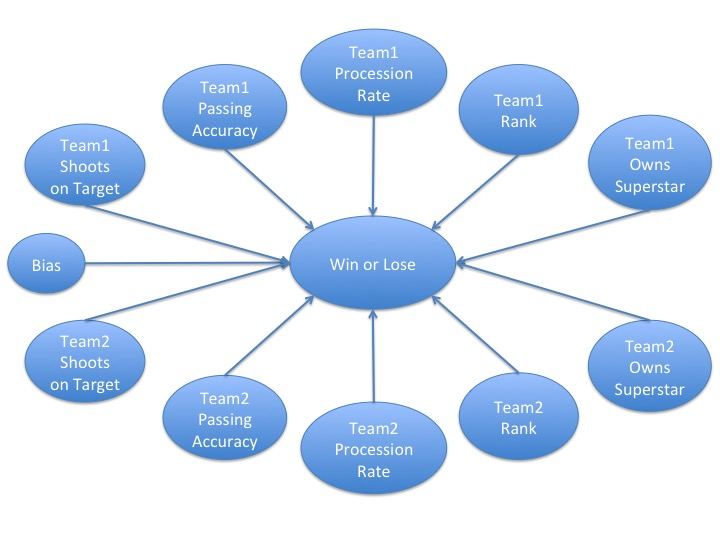
\includegraphics[width=0.9\linewidth]{graph.jpg}
\caption{Graphical Model}
\label{fig:pred}
\end{figure}

\section{Model}

We aim to establish the relationship between match results $\boldmath{y} = [y_1, \, y_2, \ldots, y_n]^T \in \mathbb{Z}^n$ and team statistics $\boldmath{X} = [\boldmath{x}_1, \, \boldmath{x}_2, \, \ldots, \boldmath{x}_p ] \in \mathbb{R}^{n \times p}$ whose columns correspond to specific statistics. Since $\boldmath{y}$ is the binary data, we propose to use the following data augmentation approach to model the data: For $i = 1, \, 2, \, \ldots, \, n$, 
\begin{eqnarray}
z_i &\sim& \mathcal{N} (z_i; \, X_i^T \boldmath{\beta}, 1)
\end{eqnarray}
where $z_i$ is the latent variable; $y_i=1 \ if \ z_i>0 \ and \ y_i=0 \ otherwise.$
Moreover, we assign the following prior on $\mathbb{\beta}$:
\begin{eqnarray}
\pi (\boldmath{\beta}) &\sim& \mathcal{N} (\boldmath{\beta}; \boldmath{\beta}_0, \, \Sigma_0 )
\end{eqnarray}

\section{Posterior Inference}

We could derive the Gibbs sampler for Bayesian linear regression as follows:
The fitted parameters $\hat{\boldmath{\beta}}$ should reflect the corresponding weights for each match statistic. We could employ the fitted $\hat{\boldmath{\beta}}$ to accomplish prediction using new dataset $\tilde{\boldmath{X}}$ as
\begin{equation}
\tilde{\boldmath{z}} = \tilde{\boldmath{X}} \hat{\boldmath{\beta}}
\label{eq:pred}
\end{equation}
\newline
A Gibbs sampler for Bayesian Linear Regression:
\newline \\
\textbf{Sampling} $\boldmath{\beta}$ from
\begin{eqnarray}
(\boldmath{\beta} | -) &\sim& \mathcal{N} ( \boldmath{\beta}; \boldmath{\hat{\beta} }, \, \hat{\Sigma} )
\end{eqnarray}
where
\begin{eqnarray*}
\boldmath{\hat{\beta}} &=& \hat{\Sigma_0} \, ( \Sigma^{-1} \boldmath{\beta_0} + \boldmath{X}^T \boldmath{z} ) \\
\hat{\Sigma} &=& ( \boldmath{X}^T \boldmath{X} + \Sigma_0^{-1} )^{-1}
\end{eqnarray*}
\textbf{Sampling} $z_i$ for $i = 1, \, 2, \, \ldots, \, n$ from
\begin{eqnarray}
(z_i | y_i=0) &\sim& \mathcal{N} ( z_i; X_i^T \boldmath{\beta}, 1 ) \{z_i\leq0\}
\end{eqnarray}
\begin{eqnarray}
(z_i | y_i=1) &\sim& \mathcal{N} ( z_i; X_i^T \boldmath{\beta}, 1 ) \{z_i>0\}
\end{eqnarray}

\section{Experimental Results}

We select five relevant variables of each team such as shoots on target, possession rate, passing accuracy, FIFA rank, the team owns superstar or not in addition to bias. We collected the game statistics of 100 elimination games of the 1998, 2002, 2006, 2010 World Cup, 2000, 2004, 2008, 2012 UEFA European Championship and 2001, 2004, 2007, 2011, 2015 Copa America into the training set. We calculate the input as the average of the historical game statistics of the two teams into the training weights we have calculated. Among the variables, we select the FIFA rank as the most influential variable that decide our prediction. The autocorrelation function and the distribution of FIFA rank are as follows.

\begin{figure}[!tbp]
  \centering
  \begin{minipage}[b]{0.4\textwidth}
    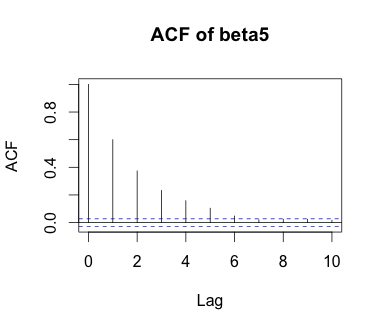
\includegraphics[width=\textwidth]{acfbeta5.png}
    \caption{Autocorrelation Function}
  \end{minipage}
  \hfill
  \begin{minipage}[b]{0.4\textwidth}
    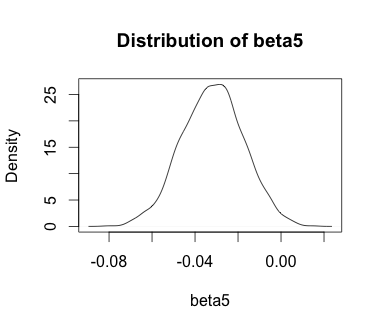
\includegraphics[width=\textwidth]{distbeta5.png}
    \caption{Density Distribution}
  \end{minipage}
\end{figure}

The final results are as follows. In the game of Columbia vs Uruguay, Belgium vs USA, France vs Germany, Brazil vs Germany and Brazil vs Netherlands, we did wrong predictions according to the real data. Interestingly, some teams even win the game with the disadvantage in all fields.

\begin{figure}[H]
\centering
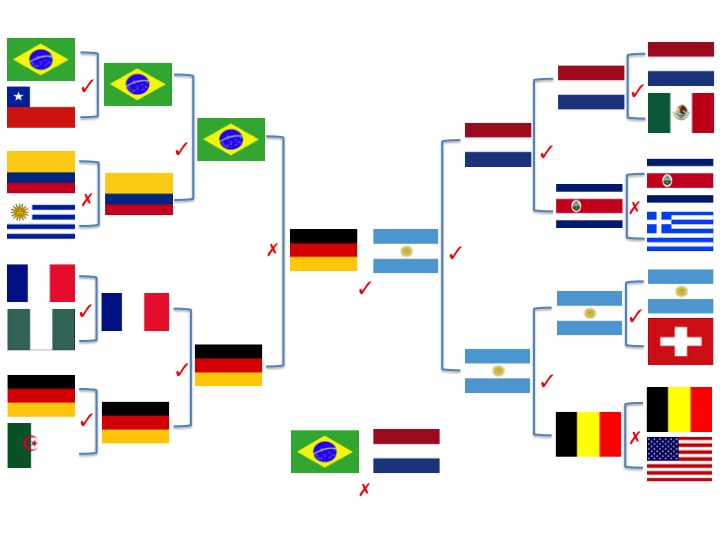
\includegraphics[width=0.9\linewidth]{Slide3.jpg}
\caption{Comparison with 2014 FIFA World Cup Bracket}
\label{fig:pred}
\end{figure}



\begin{table}[H]
\centering
\vspace{2ex}
\begin{tabular}{l l l}
\toprule
\textbf{Correct} & \textbf{Wrong} & \textbf{Accuracy}\\
\midrule
11 & 5 & 68.75\% \\
\bottomrule
\end{tabular}
\caption{Prediction Outcome}
\end{table}

\section{Further Thought}

We plan to apply some non-linear algorithms to make the prediction, like non-linear SVM and Gaussian process regression models to see if these alternatives can do better than Bayesian linear regression by comparison. 

In addition, if we analyze the five games we predicted wrong, we conclude that some team has better offensive statistics while they have worse defensive statistics than the other team. Also, the variables we selected from the game report are all about offense rather than defense. We think this is more likely to be the reason that we predicted wrong. Especially in the elimination games of World Cup, defense sometimes carries more weight than offense. 

Furthermore, there are so many variables that we cannot model. For example, in the quarterfinal, Brazil 1:7 Germany and lost to Netherlands with 0:3 in the third place game. Brazil encountered a very depressing result in the game with Germany and obviously lost the motivation to play the third place game. These two games were out of expectation because Brazil have larger advantage in all aspects. There are also situations with sudden accidents such as red card, penalty kick and severe injuries. However, maybe that is also the beauty of the World Cup. You cannot explicitly model all the variables such as spiritually variables and sudden accident variables of the whole game.

\section{Conclusion}

In the game of Columbia vs Uruguay, Belgium vs USA, France vs Germany, Brazil vs Germany and Brazil vs Netherlands, we did wrong predictions according to the real game result. Interestingly, some teams even win the game with the disadvantage in all fields. In general, we made 11 right predictions out of 16 elimination games. 

This model introduces latent parameter for making prediction. In our model, we establish the relationship between match statistics in each soccer team and the result of a match. For our method, we implement the Gibbs sampling to perform the posterior inference. The experimental results tell us that the models can fit the data well and provide the reasonable prediction.

\section{Acknowledgement}

We would like to express our special thanks of gratitude to our instructor (Sayan Mukherjee) who gave us the opportunity to do this interesting project of the World Cup topic as well as many support and help in the process of our project. This project combined the passion of two soccer fans and machine learning techniques. In the process of exploration, the project helped us have a deep understanding of machine learning inferences on real-world situations. 

\begin{thebibliography}{99}
\bibitem{ref1} Alexander Spermann. \textit{The Probit Model, University of Freiburg}. Sose, 2009.
\bibitem{ref2} Peter D Hoff. \textit{A first course in Bayesian statistical methods}. Springer, 2009.
\end{thebibliography}


\end{document}
